\chapter{The Play}

(This is for now on hiatus, due to the fact that the C:DDA Launcher ate my savefile and the game at hand actually changed a bit in terms of difficulty - I'm keeping this section for now mostly due to the fact that it does serve as a pointer, even as an unfinished one, to give directions to newcomers. At some point this will be revised and replayed.)

While in the earlier topics we did nothing but describe all the different mechanics, all the different systems and things you will come across from the start of a character to the ingame screen or guiding you along the lines of what you should and shouldn't do, this seemed a bit dry and not too practical to be put to use. However, this section, played by me, will take into consideration all the things we discussed as well my own experience (which, sadly, I cannot teach you) in the game to challenge the world of Cataclysm. This 'Play', much like a Let's Play - except in text form - for early, mid and late game is focused around one playthrough with which I hope to give you an insight of what you should do, what you should avoid, and hopefully I might as well entertain you. Why bother with it you might ask - simple. I want to show that the things I talked about in the earlier chapters matter and to validate this Tutorial, at least as much as one playthrough by an experienced player can be considered validation when we use terms like the stages in such a wide brush. I decided to go with a journal-like approach simply because besides teaching something, I also want to keep your interest high, as it might have been a bit dry to read up until this point. So I'm going to give my input, on what I'm actually looking for, what I should work towards and so on and so forth. At each appropriate stage, I will recount the progress as well as our next goal.

If you are looking for a more sophisticated Cheat Sheet as to what you should do in the various stages of the game, read one chapter beforehand.

Just as a reference, for writing these guides, as well as a guideline, I am going to start out using my beginner character earlier presented in this book in a standard world with Wander Spawns enabled:

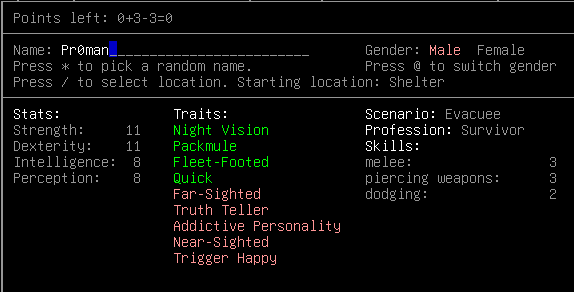
\includegraphics[width=\textwidth]{06}

For personal preference you are more than welcome to swap out anything you like, but I feel that from a combat-standpoint, this character can hold his own well, while also taking a weapon choice that is pretty good to start out with - though may be a bit annoying to craft unless you specifically head for it first.

\section{The Early Game}

So, we spawn into the world with our character, prepared to get our ass handed to us. First of all, let's check the map by pressing [m] - we need to assess the situation and see what should be the priorities:

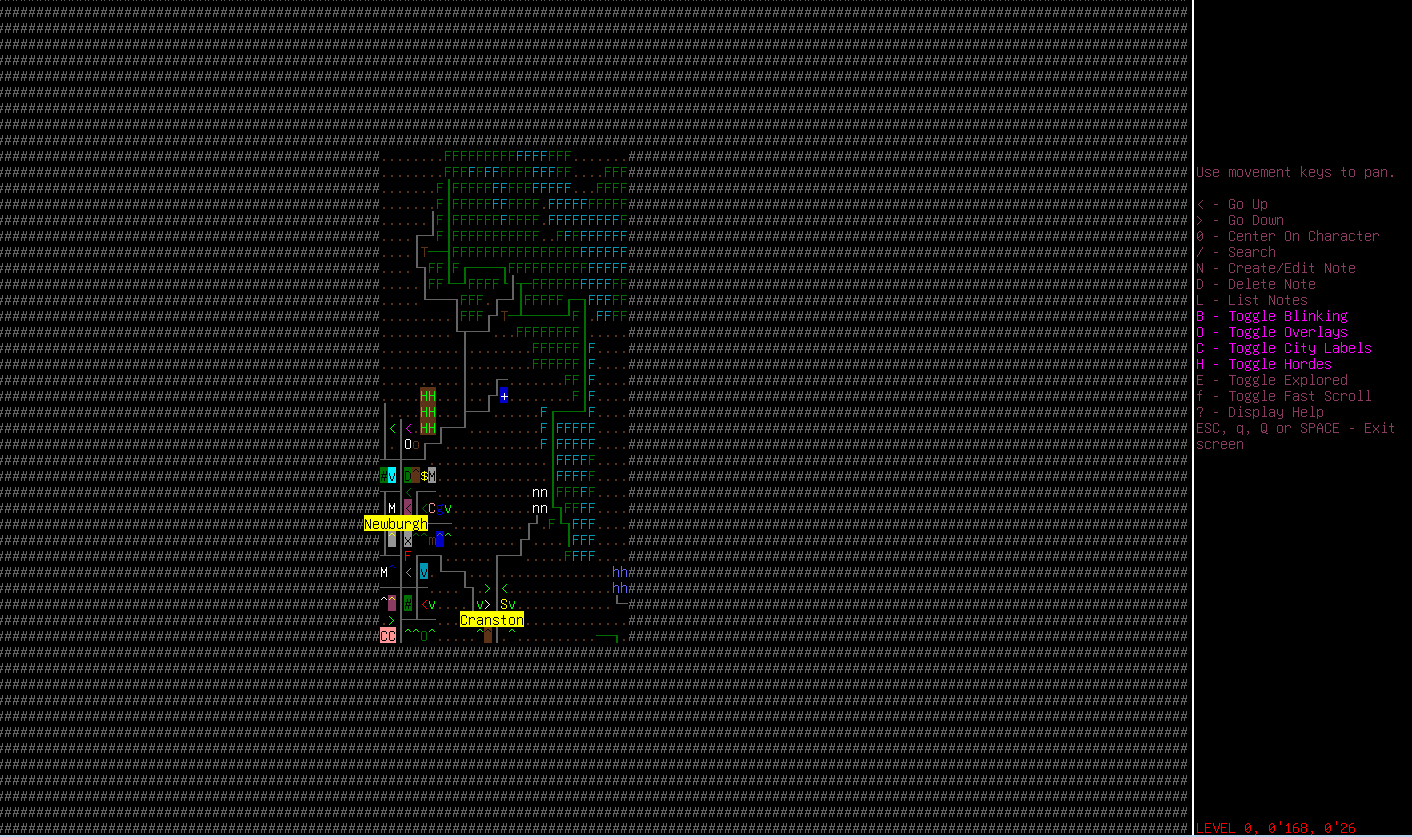
\includegraphics[width=\textwidth]{07}

As we can see, we spawned close to forests and swamps, which are intertwined with forest trails and relatively close to two cities, with some interesting structures in them - namely two libraries are visible.

However, this does not have to bother us yet. The most important things for survival are:
Water,
food,
gear,
in this order. So let us explore the shelter thoroughly.
A quick glance at the Terminal can however provide a bit of insight, we should definitely check it out and select the 'Contact Us' option so that we get a marker as to where the closest Refugee Center is, as well as a road marked towards it, if it is reachable by road.

The lockers can contain gear and utility items, mostly gas masks, first aid kits, emergency jackets and folded emergency blankets, while the basement usually contains a couple cans of food or random clothing, rarely some tools.

I got lucky in that I found a Jacket, Gas Mask and a Blanket - this will definitely keep me warm during the night.

The basement however, contained nothing at all, so, to secure water there are several options one can take - either sneak (or barge) into town, looking for cooking utensils like a pot or frying pan, as well as some containers to boil and store water gotten from the forest. Or, you could forage your survival up, hopefully find a can/bottle that has boiling quality and do pretty much the same. Since I play with wander spawns enabled, this is probably the safest option, as towns tend to spawn in lots of zombies and while my gear keeps me warm for the most part, it doesn't cover me in its' entirety and I will end up getting slowed sooner or later.

And just a couple steps to the north, right outside my shelter I already spot something:

\begin{center}
    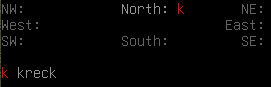
\includegraphics[width=0.5\textwidth]{08}
\end{center}

A kreck, not too difficult, but could at least damage my gear, however - and this is the important bit, where there are extra dimensional beings, there's loot to be had.

However, seems like there's more than just a Kreck, instead, a Mi-Go is right behind it. This is most definitely a fight I am not willing to risk. Those things hit hard, quite fast and you most likely will be unable to outrun them - that loot will have to wait.
So for now, let's head east instead, towards the swamp and see what we find - OH FUCK ME. A second Mi-Go.

\begin{center}
    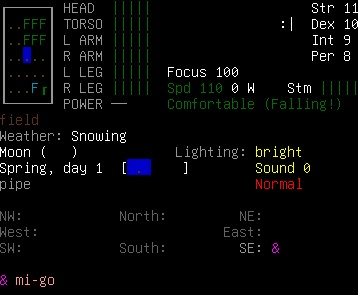
\includegraphics[width=0.5\textwidth]{09}
\end{center}

And while that may mean more loot, it means more places I need to tread extremely carefully, otherwise this run will end extremely quickly.

Well, I managed to sneak past it NE into the forest, after foraging to nearly rank 2 in survival and having no luck besides finding some veggies every now and then, I accidentally get too close to the first encounter location and aggro the Mi-Go. After a short run through the forests, I decide to try lighting a Bush on fire and to stand tall, or die here.

Lucky me, I survived' barely, my gear is messed, my head just as much, but I managed to deter the Mi-Go so it runs away in terror. It could've gone either way with the way Mi-Go's hit. So I just got lucky, this would've been a run-ender already. On the other hand, I can now loot the location.

Well, I found another plastic bottle of clean water - that will at the very least keep me going for yet another day, some Science IDs, which will definitely come in handy later, all that clothing on these 'overmap encounters' is also considered clean and comes with a decent amount of pockets. While I would always advise against going over encumbered, there isn't much I can do at this point but to grab all the things I can and hope for the best.

So in order for my vegetables and eggs to not rot away, I store them in the cellar and drop of the gear I collected somewhere (Certain foods go mushy if frozen and thawed, then rot away if frozen and thawed again)

On the other hand, I did manage to find some Rhubarb while foraging, this is totally fine to eat raw and comes with a nice bonus to our health stat (+3 each bite). That Trailhead [brown T] on the overmap might be worthwhile checking, as I spotted a car there'

Yup, there's a car there, a nice Pickup truck - lacks wheels though (and has a faulty engine, but nothing too bad), and on the radar I spot something next to it that looks like an RV.

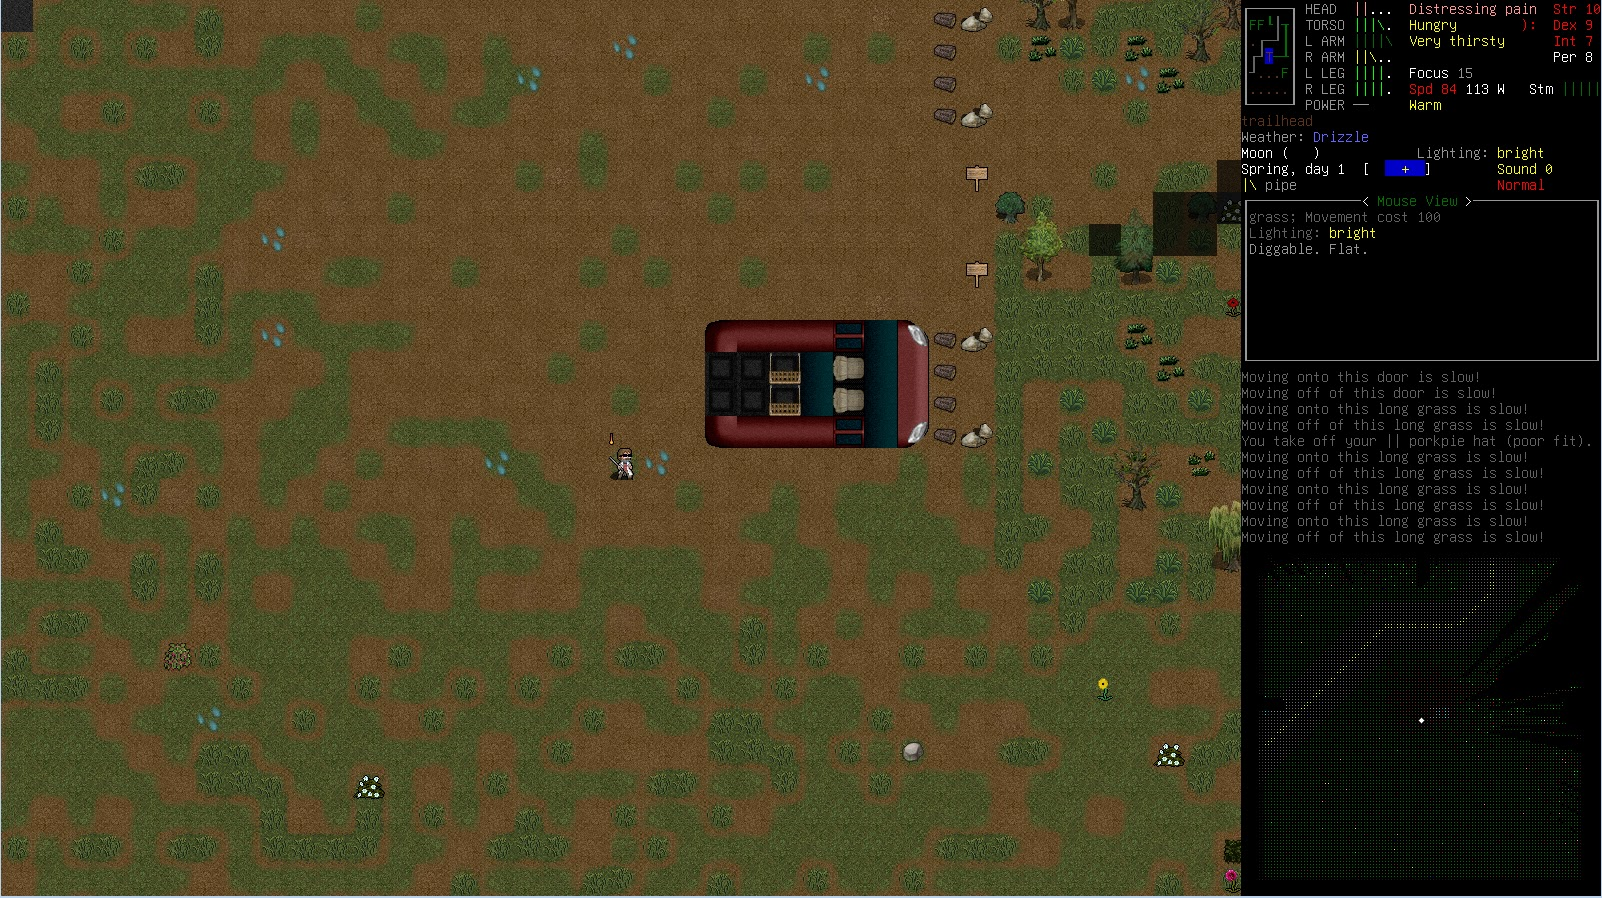
\includegraphics[width=\textwidth]{10}

Actually a meth lab, with a functioning chemistry lab. But it has no battery whatsoever inside, so no easy cooking for me. Guess it's up to more foraging and hoping for the best, as this is the only thing I can do now that I'm this beat up.

After foraging tile over tile in hopes of actually finding something with boiling quality, I decided to check out the forest trails for a bit, and look there, a glass bottle, I'm saved. Water is therefore ticked off of the list - why? Because A glass bottle is not just a container, but also able to be used to boil water in and with the 2 plastic bottles I found earlier, I also have a place to store it.

Well, it's getting dark - I basically wasted the first day looking for a suitable container to boil water with, which is nice, but it took so long and cost me lots of my HP that I'm gonna be hindered badly going forward, maybe. So, by cutting up some sheets that i tore down from the windows ([e]xamine), I craft myself some bandages till I hit tailoring of 1. Might as well go for it and apply them on each body part to gain some extra HP overnight. Before heading to bed, I'm gonna snack on the rhubarb I found earlier and have a drink to have a potentially easier time sleeping. And so I do and all of a sudden, I'm healed back to full, despite being torn up when heading to bed.

The next thing to work towards will be food supplies - while I did find lots of vegetables, eating those raw would be pretty bad for my mood, yet I can't cook them easily since they require Food cooking quality 2 to be turned into cooked wild vegetables. So, I need a better cooking utensil. Time to grab my bottles and head to a water source tile inside the forests'

By boiling water I can increase my cooking to 1, which in turn with my survival of 2 allows me to craft a stone pot, which is just barely enough and hey - I even managed to make that on my first try, even better. Time to cook some veggies. While I would prefer to have an indoor cooking place, a fire outside my shelter will have to do, as the floor is flammable and I don't want to torch down my only shelter.

(Sadly, the food rebalance update gimped this strategy of using wild veggies to keep your belly full. Making scrambled/boiled eggs works fine though.)

Now with both water and food achieved, time to work on my gear, which means, I will have to work on my skills. After [s]macking up some benches I have enough nails and splintered woods to craft not only fishing hooks till I hit fabrications 1, but improvised fishing hooks till I am at fabrications 2, great start. A wooden needle for some sewing and our first proper weapon - a wooden spear. For that we need some long stick, so just smash a young tree till you get one after it is destroyed. The long strings from the curtains provide the thread from disassembling them into small strings and thread afterwards, rags come from the same curtains and a fire, like with cooking, we will gain by lighting up a splintered wood outside of our shelter (make sure there is 2 spaces in between you and the wall, you wouldn't want the fire to accidentally spread)

Time to work on some clothing, as what we currently wear is' well, less than optimal:

\begin{center}
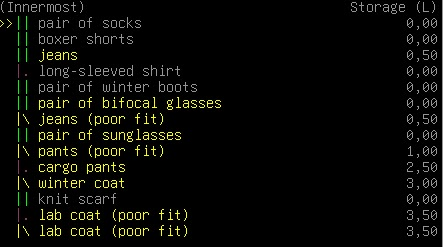
\includegraphics[width=0.5\textwidth]{11}
\end{center}

Yeah, that requires some work. good thing we made that needle and the bandages, with tailoring 1, we should have a somewhat easier time getting some gear up and running. So we grind our tailoring to 2 using pairs of light gloves (or any other recipe, it's all up to you) and at rank 2 we should definitely  make a long underwear top since that is close to the skin and therefore a great piece of clothing to wear as well as a balaclava to increase head and mouth temperature.

To grind further, I'd suggest using the T-shirt recipe, since that can also be disassembled instead of cut up, returning the full crafting resources.

Pr0-Tip: if you fail a couple of crafts, don't sweat it, the shelter has generally enough sheets to keep you outfitted for the first crafts that you do.

But why tailoring 3? Is clothing that important? Well, it is important in a sense that you require some pockets to store all the phat loots in, while also being free enough to be a force in combat, yet also not freezing to death. A clothing combo I'd suggest is a long underwear top, Duster and Backpack, Balaclava + boonie hat, some form of pants and respective boots. (the winter boots you spawn in quickly will turn your feet warm)

While sleeping, a zombie Cop decided it's time for an unannounced house search. So I promptly greeted him with my new wooden spear and he was so kind to leave me an AR-15 behind, oh goodie. While it's a bit dented, it will definitely come in handy.

Pr0-Tip: Remember that most spear-type weapons can be [f]ired in order to perform a ranged attack over 1 tile. The extra reach is what makes it for spears, while the armor piercing is more than welcome against semi-armored targets.

And on the start of day 3, this is how the clothing situation is now looking:

\begin{center}

\includegraphics[width=0.5\textwidth]{12}
\end{center}

Well, I'm pretty happy with how things turned out. And since we are now properly equipped it's time to go exploring (we traded in a bit of defense from the winter coat for way more pockets and less encumberment all around) The spear makes for a great weapon against basically anything, except the zombie Soldier, but this is simply due to its' low damage values.

Pr0-tip - whenever you manage to kill zombie enemies, remember to pulp their corpses by [s]mashing the tile the corpse lies in. This will quickly stop them from reviving by themselves. This doesn't help against necromancers, but it works for now. And if this zombie is an acidic or spitter, don't pulp them, but perform a quick butchery once the acid is gone.

But, since there are some enemies I'd wish to soften up on range and I don't feel like wasting my precious .223 remington shots from my rifle, I'm gonna quickly craft a sling out of the 3 long strings all those curtains provide. (fabrication 1) Ammo is plentiful, just craft yourself a bunch of pebbles and you are all set to use it.

Even though the sling is considered a throwing weapon, it is used like any other ranged firearm, press [f] to fire, and aim according to your own tastes.

Quickfire tutorial on ranged combat:
[f] to enter firing mode
[.] to wait a turn and therefore stabilize your aim a bit.
[f] again to fire once you feel comfortable enough and waited the for you appropriate amount of turns.
or
while in firing mode:
[a] to aim and fire (medium aim)
[c] to carefully aim and fire (pretty good aim)
[p] to precisely aim and fire (best possible aim)

What these buttons do is wait a respective amount of turns until the aiming threshold is met, at which point, you issue a fire command.

Precise aim is what I personally go for - it takes the longest time, but maxes out your aiming and waits till recoil is reduced to 0, but therefore costs the most amount of time. Why? simple, not only am I pretty accurate in gauging the distance to enemies and how far they can move while aiming with different weapons - every shot missed means I wasted turns that the enemy could use to close the gap. And later down the line, when ammo is becoming a bit more common but still just a few touches too annoying to get, I want to make every shot count.

Nevertheless - why would I go for something so abhorrently weak like the sling? Well, turns out the Romans didn't use all these slings en masse for nothing. It is actually quite powerful and takes down normal zombies in just a couple hits. With ammo being basically infinite this makes for a nice first ranged option that also levels marksmanship for later.

So now most of the normal zombies become target dummies for my sling and wooden spear and I can technically start looting and clearing out towns. however, that superstore looks awfully tempting, but usually comes at the risk of being overrun by baddies. Doesn't mean I can't go take a look.

While checking the outskirts, I notice that the amount of zombies is way too many to potentially deal with. To the forest north is a helicopter crash site, right at the edge of the forest, Besides the zombie military pilot and soldiers, which already make this place unlootable for me, there's also a zombie bio-operator, something I will HAVE to avoid, as this could be run-ending.

So I venture further west, hoping of finding a nice entry way into the town, but mostly it's brutes, shockers or acidic zombies on the outskirts, far enough to potentially squeak through, but close enough that i don't want to take the risk. While walking back it appears as though the group of soldiers dispersed from the wreckage - turns out they guarded a poor fitting army helmet and an EMP. Well, whatever works. The dog they decided to maul gets field dressed first (to receive stomachs and offal) then fully butchered and that provides me with meat to my diet, while needing to be cooked first, the stuff will come in handy, especially the bones. The stomach that I managed to butcher will be turned into a sealed stomach, more water containers is a helpful benefit this early. While walking back, I noticed that to the SW of my shelter, there's also a Kreck running around, even more extra dimensional beings. I must've pissed off some sort of god to be this boxed in.

And while collecting water from my tile N-NE, I got attacked by the Mi-Go that I scared away on day 1 (btw, I was using a pipe from a smashed locker), looks like he wanted to go for another round, but this time, it was a fight to the death, for him. Though he did do a number on me and wrecked my clothing, torso and left leg and if that ain't enough, a spitter decided to show up just as I was about to craft the stomach. After quickly disposing of him, I sat down to lick my wounds, fix my gear and boarding up those windows, these zombies get awfully close.

Lucky that I found a hammer on one of the corpses and even if that wasn't a possibility, crafting a stone hammer at this point is no big task. As I started exploring the town SW of my location, i noticed a couple more wreckages and at this point I'm left wondering - is the world generation a tad borked? we'll see. Though as soon as I noticed obstructed vision on the radar, I knew there was something producing gas or smoke nearby, and yup, it's a smoker. Time to head back and actually grab the gas mask, prepare it and keep it on hand

Man, I seem to be getting extremely bad luck. While heading back, I nearly ran into a shocker brute and a normal brute by accident, luckily though I noticed them before they did notice me, allowing me to run as quickly as I could into the opposite direction - crisis averted.

After some approaches from different angles I managed to get towards a house on the eastern side, taking out a couple zombies on the way. Finally some building to ransack. Not only did the fridge have some edibles: A gallon Jug of milk and sandwiches of various kinds. But the oven I decided to bash out with my crowbar to obtain a sheet metal that will later be turned into a brazier, something that will contain fires, allowing for indoor cooking. Not only that, but amongst other things I found some drinks, more canned food, a desk fan and Atreyupan as well as other household drugs, which will be great if I ever happen to have a bite wound but no antiseptic medication on hand.

So it is now day 5

I'm pretty well situated for where I started out as, have some gear and food stocks, now I should work on scavenging together some tools and maybe look for a vehicle that would be worthwhile turning into a base.
Another factor in 'leaving' my shelter, speak my base behind, is the fact that the shocker brute is walking awfully close to it, and he has no trouble smashing up some house walls to get to my fleshy parts.

Well, what do you know, I did technically find a car that is drivable, a simple, plain car. Comes with a pretty battered fuel tank though, so it'll most likely leak gas everywhere. But in a pinch I could just ram the Shocker brute and be done with it.

But back to looting - while checking another house, an abandoned storefront and a gambling hall, I managed to come across a charcoal smoker (pretty useful for preservation), a real pot (finally some real cooking) as well as more food and a small book. Before I knew it, there were more zombies outside, guess they must've wandered in. One of them was nice enough to provide me with a toolbox, something I will gladly take at this stage of the game, as it combines most of the tools required into 1 handy item.

While this will come in handy - my assumptions happened: the car lost its' gasoline and now I have to haul things around. So I quickly turn some sheets from nearby houses into 2 makeshift slings, grab all my belongings and venture to the Military Surplus that is on the way. Not only do I find an Army helmet that actually does fit, but also the gun owners handbook as well as a plastic canteen, so now I can wear some water container on me at all times: The potentially best find could turn out to be the Leather Jacket as well as the hunting knife, as this knife is the best possible butchery tool easily available and the Jacket provides excellent protection, being made out of leather. Guess it's time to leg it back while assessing some cars and my potential options.

While considering what to do the next day, I decided to check out the Mobile Meth lab and to my dismay, it has no fuel tank, no battery and the engine has no drive belt. While that is in itself a minor inconvenience, the missing tank requires me to find or make a welder to replace that. But on the other hand, it would make for a great vehicle, not just coming with storage, but also a great vehicular station - the Chemistry Lab. So I decided to take a peek at the superstore, and to the road south of it, what do my sore eyes see? Another meth lab, only lacking some wheels - considering a Bottle Jack is way easier to come by, I'm most likely going to claim this vehicle instead, though it might be a bit parked in. Deciding to tackle to dollar store (which I mistook for a bank at first glance) I was able to grab me a shopping cart in perfect condition, meaning I now have a way of hauling around large amounts of items no problem, as well as finding a second canteen, so now all my water container problems are basically non-existent. Since the library was next door, I decided to head there, only to find several great books - The big book of first aid, Biodiesel: the renewable fuel source, A history of Firefighting, how to trap anything, the book of dances and last but not least The historic weaponsmith(!) this will most likely proof to be extremely valuable, as this'll allow me to craft medieval weapons of all kinds that have quite the punch to them - from a Morningstar and Mace to the Estoc, Halberds, Glaives, different kinds of swords, the Awl pike (though that one was nerfed terribly as of recently). This will come in real handy real quickly. The only problem is gonna be managing to get a forge and maintaining said forge. But I might as well start working on this. The fabrications skill is easily obtainable by grinding certain crafting recipes (Distaff and Spindle - Pair of wooden Clogs - Banded wooden Cart wheel), this way, I can easily reach fabrication 5 in two days' work, while my supplies keep me covered. Drinkables are a non-issue at this point, as is food - animals in somewhat close proximity to the shelter can quickly be killed (except for moose or bears), butchered and turned into food.

So not only did we tick off the most pressing needs in form of water, food and gear (god that toolbox drop) as well as shelter - the starting evacuee shelter makes for a great makeshift base of operations to start out with, but we also managed to scout out some vehicles, are about to set up a forge to allow for some extra weapons as sidearms to switch to and can freely grind any skill we like, as not many enemies at this stage pose much of a threat, with the exception to shocker brutes and enemies bigger than that.

Due to being settled in properly, I'd suggest that this is the end point of the early game and we can say we clearly moved towards the mid game.

\section{The Mid Game}

Day 8 - not a bad situation to be in, as I not only have a toolbox, several great books to boot, a vehicle scouted out and lots of permanent food in the form of cans as well as several animals running around close to the shelter if I ever want something more fresh.

However, as I was grinding skills, a horde apparently decided to walk around my shelter as there's been several shockers in that group, one of them a brute. So, nighttime combat it is then - the spear easily deals with most of the enemies, except those electrical ones. those I take out with a sling, many pebbles and lots of dedication. At dawn I check the aftermath of the murder to loot, pulp any zombies I missed and start heading out for the next day - couple pieces of loot include:

-ammo + a single barrel shotgun
-electrical tools (flashlights, tazers, radios)
-a mini freezer (sweet)
-several drugs, aspirin, cough syrup and so on.

Since I'm wanting to make a forge setup, as I do require better weapons at this point, I'll have to collect lots of rocks, 80 at least. I'm gonna go with the safer approach of checking the forests for small boulders to bash down (1-6 rocks each), as torching a building would cause many enemies to get spawned nearby (wander spawns) and maybe stopping short of the fire, leaving the area difficult to reach.

This also has the added benefit of gaining some extra food items to eat so that I can save my permanent food items for a bit longer.

Collecting all those rocks took me a day, but depending on luck might require more time - careful when doing this at night, a moose decided to watch me.. a bit closer than I'd have liked, so I decided to poke him with my spear and turn him into edibles.

So, for a proper forge setup, we require:

-Charcoal kiln
-Rock forge
-several tools

The Kiln and forge are no problem, while we construct the forge, I also filled up the kiln with a bunch of sticks I collected from young trees outside the base.

However, now we need metal, lots of it. While having the toolbox makes this really easy to get (just remove vehicle parts like doors for frames), we can also check wreckages to see if there's already bashed out frames, as well as collecting lots of scrap. After bringing over a sufficient amount of metal in forms of frames (5), a sheet metal and lots of lumps/chunks, we can forge ourselves the tools required to operate a forge - crucible, anvil, metal tongs, metalworking chisel and a swage an die set -, an entire toolset, which we luckily won't need, and also more importantly - bigger weapons.

As for that part - I'd suggest any player to go with a Steel Spear, simply due to its superior range. Which is also what I'll be going for, as it makes dispatching shocker brutes totally possible.

Next up on the list is looting that nice home improvement Superstore next door while also cleaning that one out a bit.

And while it wasn't all too difficult all things considered, the loot was pretty worth it - lots of spare parts, mostly nails and copper wire, some utility tools like bolt cutters but by far the best loot in it was a telescopic crane mounted on a foldable frame, meaning I now have some lifting and jacking quality at hand which can be stored away nicely.

Since we did have that RV in pretty decent condition only lacking wheels, time to look around the different kinds of cars in order to find some wheels. While 32' wide wheels would be great right about now, anything will do, even some 17' normal wheels. However, to do any sort of work related to vehicles, I need skills - while I have a mechanics book for range 3 - 6, I need mechanics 3, and electronics won't hurt either, so time to just do some general looting.

Good thing there was still a library just a couple minutes walk south - in it were lots of great books, same with the surrounding housing - Mechanical Mastery, Sewing Techniques for Designers as well as the Clothing Designers Portfolio, Ham Radio Illustrated and What's a Transistor. I ought to play the game more often on easier settings, sure feels good.

Anyways, the two electronics books are quickly read, giving me access to a soldering iron, Under the hood provides me with mechanics 3, and there's the welder already, even with battery compartment mod due to one of the electronics books having it.

After stocking up on car batteries, trying to find some wheels (those must've been the first thing to get hit by the cataclysm, I had a really hard time tracking any useable wheel down) and even managing to find 3 solar panels, I decided to bring a batch of food and water with me, i'm gonna do some mechanics work.

Mostly uneventful except for the odd zombie showing interest in my finesse with the tools. Installing wheels and [c]hanging them where it's necessary sure took its time. Slapping on the solar panels that I found will at least, over time, recharge my car batteries that I'm inevitably drain using the welder. Took me two days straight to get the thing up and running, since, hell, might as well upgrade it a bit and the low-end cube van right next to it provided some sweet cargo spaces to increase my loading capacity. After I get this thing to run properly, I [s]iphon some gas from the nearby vehicles and drive back to my makeshift base, which is the evac shelter. Since I'll be planning to live on the road in order to explore many different features, we'll be abandoning this camp, so time to pack up - I made some makeshift slings and wore another backpack and went packing, sorting everything properly. Now that that's out of the way, let's get to reading up all those books. Skills matter, and if I wish to forge some weapons, an electric forge with a compartment mod is my best bet at this point. The remaining charcoal that I made will be used for the small charcoal smoker I found earlier. Good thing there was this home improvement superstore - the ovens in there will be handy to get the heating elements I need.

But like I said - skills are survival, without better combat skills I will be stuck against bigger enemies, without better armor, which I can now craft thanks to those books, I will constantly take damage and without late game power tools I will have trouble breaking and entering late game structures.

While reading, I totally did not notice that one of the books I looted appears to give me the weapon arts 'Fencing', so I guess instead of going for an Estoc, I'll make a broadsword instead as it is a compatible weapon for this style. Having multiple melee options is not a bad thing anyways. So off to more looting, resources for better armor are not just acquired overnight, at least for the most part.

While cleaning out the city I noticed some acidic soldier ants at the NW edge of town. Seems like I found myself a nice playground for the later stages of the game.

\section{The Late Game}